\documentclass[tikz]{standalone}
\usepackage{amssymb}
\begin{document}
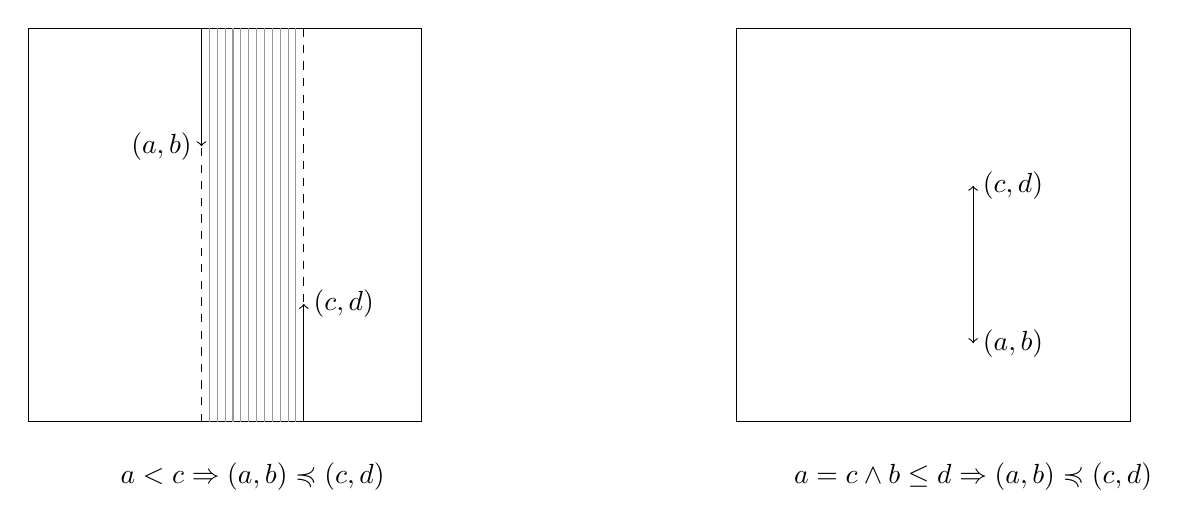
\begin{tikzpicture}
	%\filldraw[gray!20] (2.2, 0) -- (3.5, 0) -- (3.5, 5) -- (2.2, 5) -- cycle;
	\draw (0, 0) -- (5, 0) -- (5, 5) -- (0, 5) -- cycle;
	\draw[->] (2.2, 5) -- (2.2, 3.5);
	\draw[->] (3.5, 0) -- (3.5, 1.5);
	\draw[dashed] (2.2, 0) -- (2.2, 3.5);
	\draw[dashed] (3.5, 5) -- (3.5, 1.5);
	\draw (2.2, 3.5) node[left] {$(a, b)$};
	\draw (3.5, 1.5) node[right] {$(c, d)$};
	\draw (2.85, -1) node[above] {$a<c \Rightarrow (a, b) \preccurlyeq (c, d) $};
	\foreach \x in {0.1,0.2, ...,1.2}
	\draw[color=gray!80]  (2.2 + \x,0)--(2.2 + \x, 5);
	
	
	\draw (9, 0) -- (14, 0) -- (14, 5) -- (9, 5) -- cycle;
	\draw[<->] (12, 1) -- (12, 3);
	\draw (12, 1) node[right] {$(a, b)$};
	\draw (12, 3) node[right] {$(c, d)$};
	\draw (12, -1) node[above] {$a = c \wedge b \leq d \Rightarrow (a, b) \preccurlyeq (c, d) $};

  %\draw (0,0)--(1.2,0)--(1.2,1.2)--(0,1.2)--cycle;
 % \draw[color=black, very thick]  (0,0)--(0,1);
 % \draw[color=black, very thick]  (0,0)--(1,0);
	%\foreach \x in {1, ..., 90}
	%\draw[color=black]  (0,0)--(5,5/\x);
	
% \filldraw[red] (5, 0) circle (2pt);
\end{tikzpicture}
\end{document}